\documentclass[12pt]{article}
\usepackage{amsmath}
\usepackage{amssymb}
\usepackage[letterpaper,margin=0.85in,centering]{geometry}
\usepackage{fancyhdr}
\usepackage{enumerate}
\usepackage{lastpage}
\usepackage{multicol}
\usepackage{graphicx}

\reversemarginpar

\pagestyle{fancy}
\cfoot{}
\lhead{Math 1410}\chead{Worksheet \# 2}\rhead{September 21/22, 2016}
%\rfoot{Total: 10 points}
%\chead{{\bf Name:}}
\newcommand{\points}[1]{\marginpar{\hspace{24pt}[#1]}}
\newcommand{\skipline}{\vspace{12pt}}
%\renewcommand{\headrulewidth}{0in}
\headheight 30pt

\newcommand{\di}{\displaystyle}
\newcommand{\abs}[1]{\lvert #1\rvert}
\newcommand{\len}[1]{\lVert #1\rVert}
\renewcommand{\i}{\mathbf{i}}
\renewcommand{\j}{\mathbf{j}}
\renewcommand{\k}{\mathbf{k}}
\newcommand{\R}{\mathbb{R}}
\newcommand{\aaa}{\mathbf{a}}
\newcommand{\bbb}{\mathbf{b}}
\newcommand{\ccc}{\mathbf{c}}
\newcommand{\dotp}{\boldsymbol{\cdot}}
\newcommand{\bbm}{\begin{bmatrix}}
\newcommand{\ebm}{\end{bmatrix}}                   
                  
\begin{document}


\bigskip

%\author{Instructor: Sean Fitzpatrick}
\thispagestyle{fancy}
%\noindent{{\bf Name and student number:}}

 \begin{enumerate}
 \item Calculate the four 4th roots of the complex number $z=-2\sqrt{3}+2i$.

\medskip

Writing $z$ in polar form, we have $z=4\left(-\dfrac{\sqrt{3}}{2}+\frac{1}{2}i\right) = 4e^{i(5\pi/6)}$. If $w$ is a 4th root of $z$, then $w^4=z$. Writing $w=re^{i\theta}$, we have $w^4 = r^4e^{i(4\theta)} = 4e^{i(5\pi/6)} = z$.

Comparing these two numbers, we have $r^4=4$, so $r=\sqrt[4]{4} = \sqrt{2}$, and (since we can add any multiple of $2\pi$ to the argument $5\pi/6$ without changing the value of $z$) $4\theta = \dfrac{5\pi}{6}, \dfrac{17\pi}{6}, \dfrac{29\pi}{6}, \dfrac{41\pi}{6},\ldots$

Dividing by 4, we get the values $\theta = \dfrac{5\pi}{24}, \dfrac{17\pi}{24}, \dfrac{29\pi}{24}, \dfrac{41\pi}{24}$, (the next value is $\dfrac{53\pi}{24}=\dfrac{5\pi}{24}+2\pi$, and things continue repeat from there) so the four roots are
\[
 w_0 = \sqrt{2}e^{i(5\pi/24)}, w_1 = \sqrt{2}e^{i(17\pi/24)}, w_2 = \sqrt{2}e^{i(29\pi/24)}, \text{ and } w_3 = \sqrt{2}e^{i(41\pi/24)}.
\]



 \item  Let $P=(1,0,-2)$, $Q=(-3,2,4)$, and $R=(0,5,-1)$ be points in $\R^3$.
\begin{enumerate}
 \item Calculate the vectors $\vec{u}=\overrightarrow{PQ}$, $\vec{v}=\overrightarrow{QR}$, and $\vec{w}=\overrightarrow{PR}$.

\medskip

We have 
\begin{align*}
\vec{u} & = \langle -3-1,2-0,4-(-2)\rangle = \langle -4,2,6\rangle\\
\vec{v} & = \langle 0-(-3),5-2,-1-4\rangle = \langle 3,3,-5\rangle\\
\vec{w} & = \langle 0-1, 5-0, -1-(-2)\rangle = \langle -1,5,1\rangle.
\end{align*}


 \item Check that $\vec{u}+\vec{v} = \vec{w}$.

\[
\vec{u}+\vec{v} = \langle -4,2,6\rangle+\langle 3,3,-5\rangle = \langle -1,5,1\rangle = \vec{w}.
\]

\medskip

 \item Explain, with a diagram, why your result in part (b) makes sense. (You do not have to accurately plot the points $P,Q,R$.)

\bigskip

Any diagram showing the three points, labelled $P,Q,R$, and the vectors between them, will do. The point is to notice that the vector from $P$ to $R$ is the same as the vector obtained by applying the ``tip-to-tail'' rule for adding vectors. The vector $\vec{u}+\vec{v}$ also gets us from $P$ to $R$, but takes a detour through the point $Q$ along the way.
\end{enumerate}
\newpage

\item Let $\vec{a} = \langle 2,-4,3\rangle$, $\vec{b} = \langle -5, 2, 7\rangle$, and $\vec{c} = \langle 1,0,-3\rangle$. Calculate the following:
\begin{enumerate}
 \item $4\vec{a}-3\vec{b}$

\[
 4\vec{a}-3\vec{b} = 4\langle 2,-4,3\rangle-3\langle -5,2,7\rangle = \langle 8,-16,12\rangle + \langle 15, -6,-21\rangle = \langle 23,-22,-9\rangle.
\]


 \item $\len{3\vec{c}}$

\medskip

We have $3\vec{c} = 3\langle 1,0,-3\rangle = \langle 3,0,-9\rangle$, so
\[
 \len{3\vec{c}} = \len{\langle 3,0,-9\rangle} = \sqrt{3^2+0^2+(-9)^2} = \sqrt{90}.
\]


 \item $3\len{\vec{c}}$

\medskip

We have $\len{\vec{c}} = \sqrt{1^2+0^2+(-3)^3} = \sqrt{10}$, so $3\len{\vec{c}} = 3\sqrt{10}$. Note that this is the same value as the previous answer: $\sqrt{90}=\sqrt{9\cdot 10}=3\sqrt{10}$.

\medskip

 \item $\vec{a}\dotp (2\vec{b}-\vec{c})$

\medskip

Since $2\vec{b}-\vec{c}  = \langle -10,4,14\rangle - \langle 1,0,-3\rangle = \langle -11,4,17\rangle$, we have
\[
 \vec{a}\dotp (2\vec{b}-\vec{c}) = \langle 2,-4,3\rangle\dotp \langle -11,4,11\rangle = 2(-11)-4(4)+3(17) = 13.
\]


 \item $2(\vec{a}\dotp \vec{b}) - \vec{a}\dotp\vec{c}$

\medskip

We have
\begin{align*}
 \vec{a}\dotp \vec{b} &= 2(-5)-4(2)+3(7) = 3 \text{ and}\\
 \vec{a}\dotp \vec{c} &= 2(1)-4(0)+3(-3) = -7,
\end{align*}
so $2(\vec{a}\dotp \vec{b}) - \vec{a}\dotp\vec{c} = 2(3)-(-7) = 13$, which is the same as the previous value.

\end{enumerate}

\item Referring to the diagram below, argue that the indicated distance $d$ is given by $d = \dfrac{\vec{a}\dotp\vec{b}}{\len{\vec{a}}}$.

\bigskip

\begin{multicols}{2}
\begin{flushleft}
 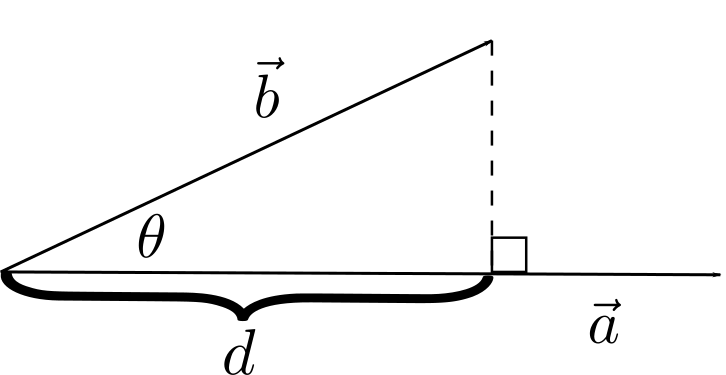
\includegraphics[width=2in]{WS2_proj}
\end{flushleft}
\columnbreak

Since $\len{\vec{b}}$ is the length of the hypotenuse of the right-angled triangle shown, we have $\cos\theta = \dfrac{d}{\len{b}}$, and thus $d=\len{\vec{b}}\cos\theta$. We also know that $\vec{a}\dotp\vec{b} = \len{\vec{a}}\len{\vec{b}}\cos\theta$, so $\cos\theta = (\vec{a}\dotp \vec{b})/(\len{\vec{a}}\len{\vec{b}})$. Thus,
\[
 d = \len{\vec{b}}\cos\theta = \len{\vec{b}}\left(\frac{\vec{a}\dotp \vec{b}}{\len{\vec{a}}\len{\vec{b}}}\right) = \dfrac{\vec{a}\dotp\vec{b}}{\len{\vec{a}}},
\]
as required.
\end{multicols}



 \end{enumerate}\end{document}